\section{Thursday, August 25th}
\subsection{Class Syllabus}

\subsubsection{Lectures}
Lectures will be in-person, TuTh 2-4pm in North Gate 105. Lectures will be recorded.

Please do not come to lecture if you have COVID symptoms; watch the recording instead!

\subsubsection{Course Staff and Communication}

Here is the EE 120 course staff for this semester!

Babak Ayazifar: Professor (ayazifar@berkeley.edu, 517 Cory)

Naomi Sagan: Head TA

Drake Lin: TA

Neerja Aggarwal: TA

Yousef Helal: TA

FourierBot: Bot

All course communication will be through Ed and BCourses (we do not have a course website).

For emergency communication during exams, email ee120-fa22@lists.berkeley.edu with [EE 120] in the subject header. This reaches all course staff.

For administrative concerns, email Naomi (naomi.sagan@berkeley.edu) and/or Babak (ayazifar@berkeley.edu) with [EE 120] in the subject header.

\subsubsection{Exams}

We will have one quiz and two midterms (no final). Exams will be online, non-proctored, open-book, and open-note during class time. You are allowed to collaborate with others. Stay tuned for more information (including exam dates) in the main logistics post!

\subsubsection{Assignments}

We will typically have one homework or lab (i.e., Jupyter notebook assignment) per week, except exam weeks. There are approximately 6-8 total homeworks, and 5 labs. For homework, the lowest two grades are dropped, and for lab, the lowest one is dropped.

Assignments will be released on Fridays and due the following Friday at 11:59pm. There will be a grace period until Sunday at 11:59pm.

Homeworks will be self-graded, and self grades will be due a week after the homework is due. Labs will be autograded, and some may have a self-graded component.

You will all be added to Gradescope shortly, by the time the first assignment is released.

\subsubsection{Discussion and OH}

Discussion Times: Friday 10-11am in Cory 521, 1-2pm in Wheeler 130, 2-3pm in Wheeler 224, 3-4pm in Wheeler 224. You can attend any section that isn't oversubscribed.

The first discussion will be Friday, August 26.

OH times are TBD; more information will be posted next week. OH will be a combination of in-person and hybrid. 

We will have homework party Friday evening, 5-6pm.

OH and homework party start the week of August 29.

\subsubsection{Course Materials}

There is no official textbook or set of course notes for EE120. However, if you would like additional information beyond what is covered in lectures, homeworks, and labs, you can look at these two textbooks:
\begin{itemize}
    \item Signals and Systems by Oppenheim and Willsky
    \item Signals and Systems by Hwei P. Hsu
\end{itemize}

To study, you should do old exams on \url{https://tbp.berkeley.edu/courses/ee/120/}.


\newpage
\subsection{Overview}
This class looks at 2 duality's:
\begin{itemize}
    \item Time $\leftrightarrow$ Frequency
    \item Continuous Time (CT) and Discrete Time (DT)
    \begin{itemize}
        \item Real-valued CT Signal: $x: \mathbb{R}\to\mathbb{R}$
        \item Complex-valued DT Signal: $x: \mathbb{Z}\to\mathbb{C}$
    \end{itemize}
\end{itemize}
The fundamental mathematical idea in this class is \textbf{signals}, and \textbf{systems} are relationships between signals.

\subsection{Signals}

\textbf{Signals are functions.}
\\
We can define signal $x$ as a function/mapping between sets $A$ and $B$: \\
\[
\tikzmark{signal}x: \tikzmark{A}A \to \tikzmark{B}B
\] 
\begin{tikzpicture}[remember picture,overlay]
\draw[<-] 
  ([shift={(2pt,10pt)}]pic cs:signal) |- ([shift={(10pt,15pt)}]pic cs:signal) 
  node[anchor=west] {Name};
\draw[<-] 
  ([shift={(2pt,-2pt)}]pic cs:A) |- ([shift={(-10pt,-10pt)}]pic cs:A) 
  node[anchor=east] {Domain};
\draw[<-] 
  ([shift={(2pt,-2pt)}]pic cs:B) |- ([shift={(14pt,-10pt)}]pic cs:B) 
  node[anchor=west] {Co-Domain};
\end{tikzpicture}

\textbf{For Discrete-Time (DT) Signals}, $A \subseteq \mathbb{Z}$ and $B \subseteq \mathbb{R} \text{ or } \mathbb{C}$.

\textbf{For Continuous-Time (CT) Signals}, $A \subseteq \mathbb{R}$ and $B \subseteq \mathbb{R} \text{ or } \mathbb{C}$.

\subsubsection{Example 1: DT Signal}
\begin{center}
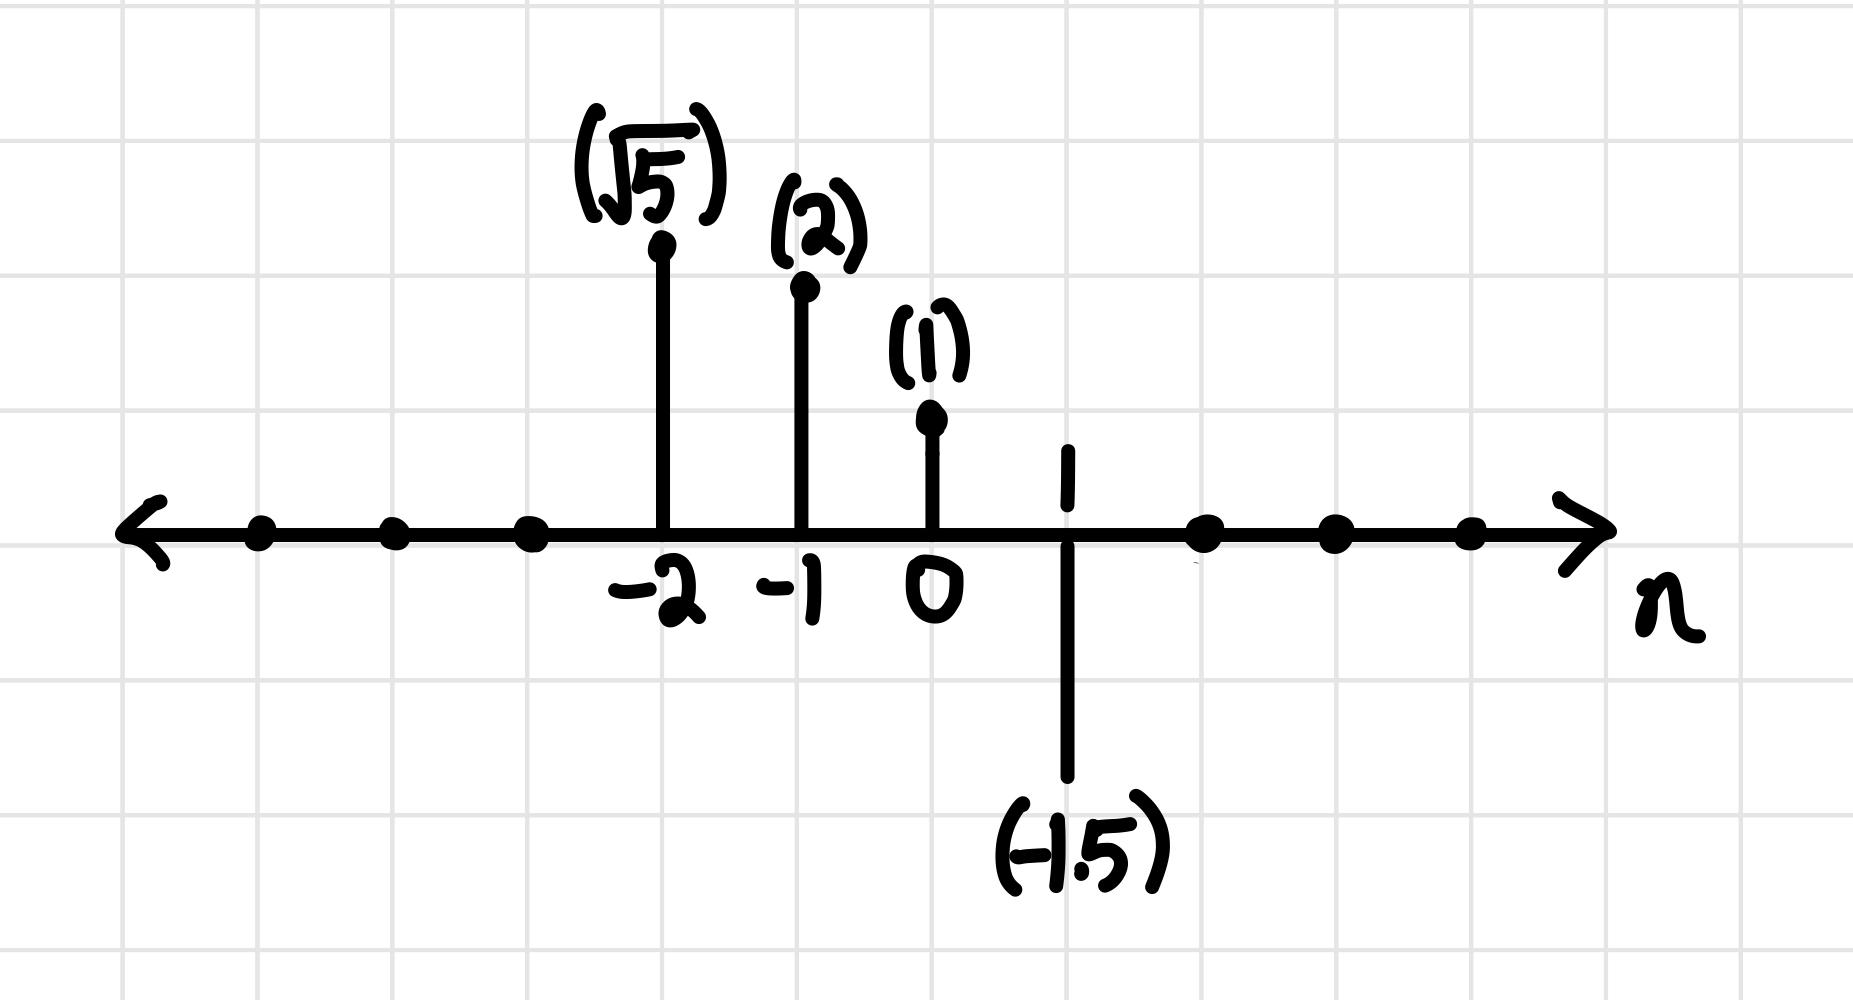
\includegraphics[ width=\textwidth/2]{lectures/img/Lec1_1.jpeg}
\end{center}

\begin{align*}
    x&: \text{function (signal in its entirety)}\\
    x(n)&: \text{value of the function $x$ evaluated at sample $n$}
\end{align*}
Thus, we have
\begin{align*}
    x(-2) &= \sqrt5 \\
    x(0.5) &= \text{undefined}
\end{align*}

\subsubsection{Example 2: CT Signal}
\begin{center}
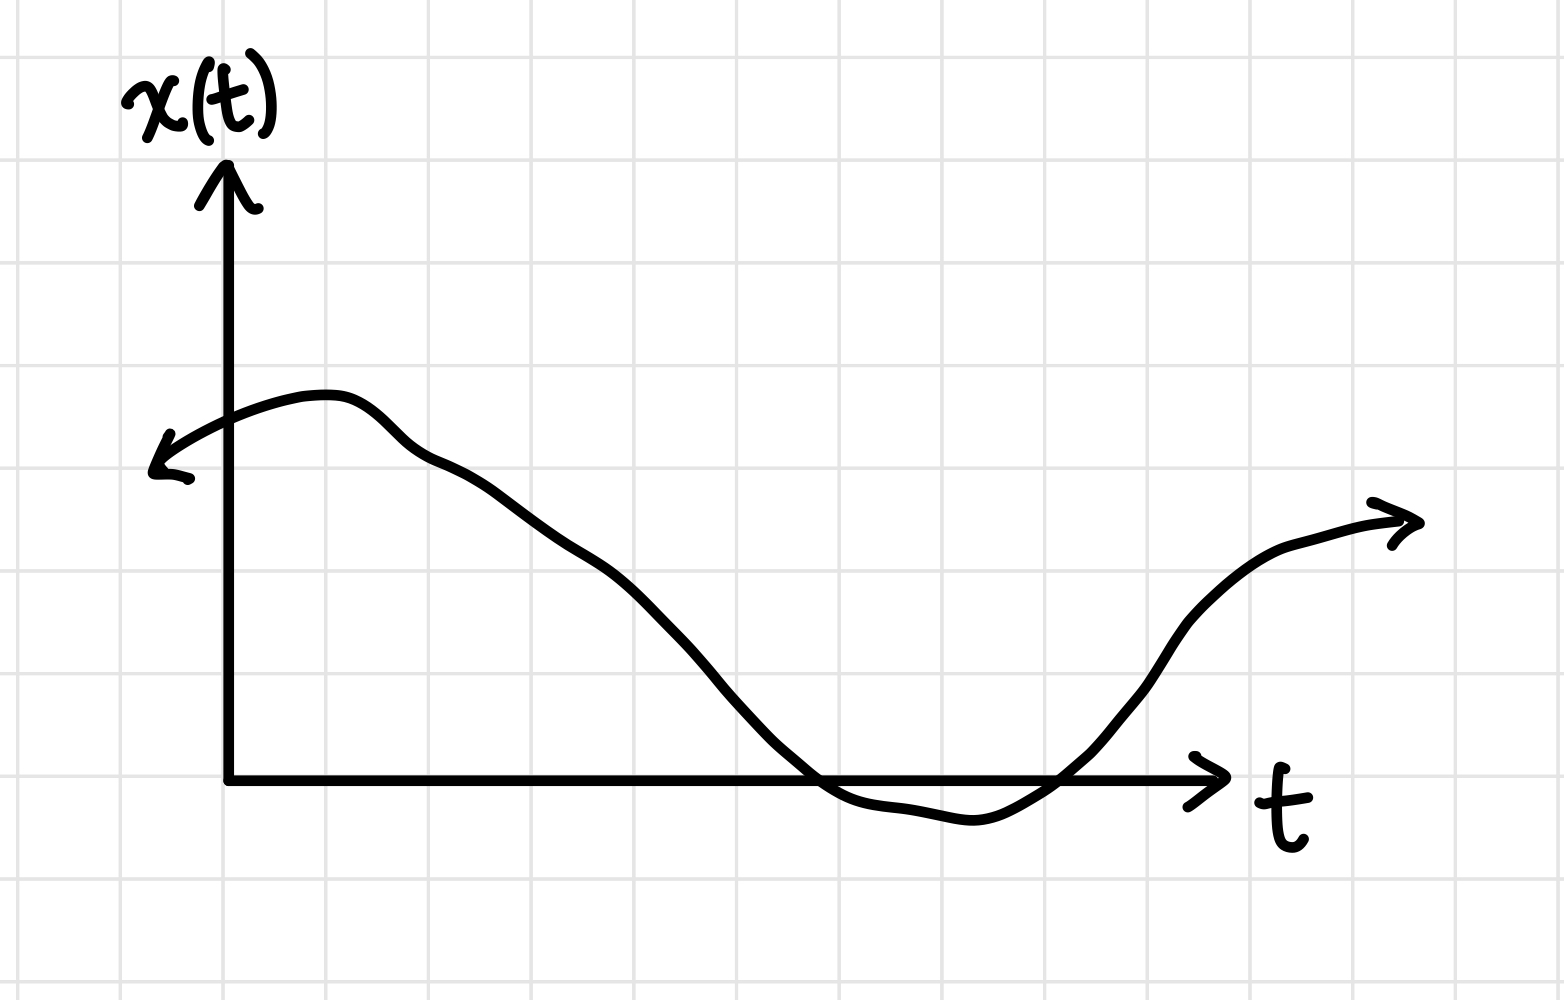
\includegraphics[ width=\textwidth/2]{lectures/img/Lec1_2.jpeg}
\end{center}

\subsubsection{Kronecker Delta (DT Impulse)}

\begin{center}
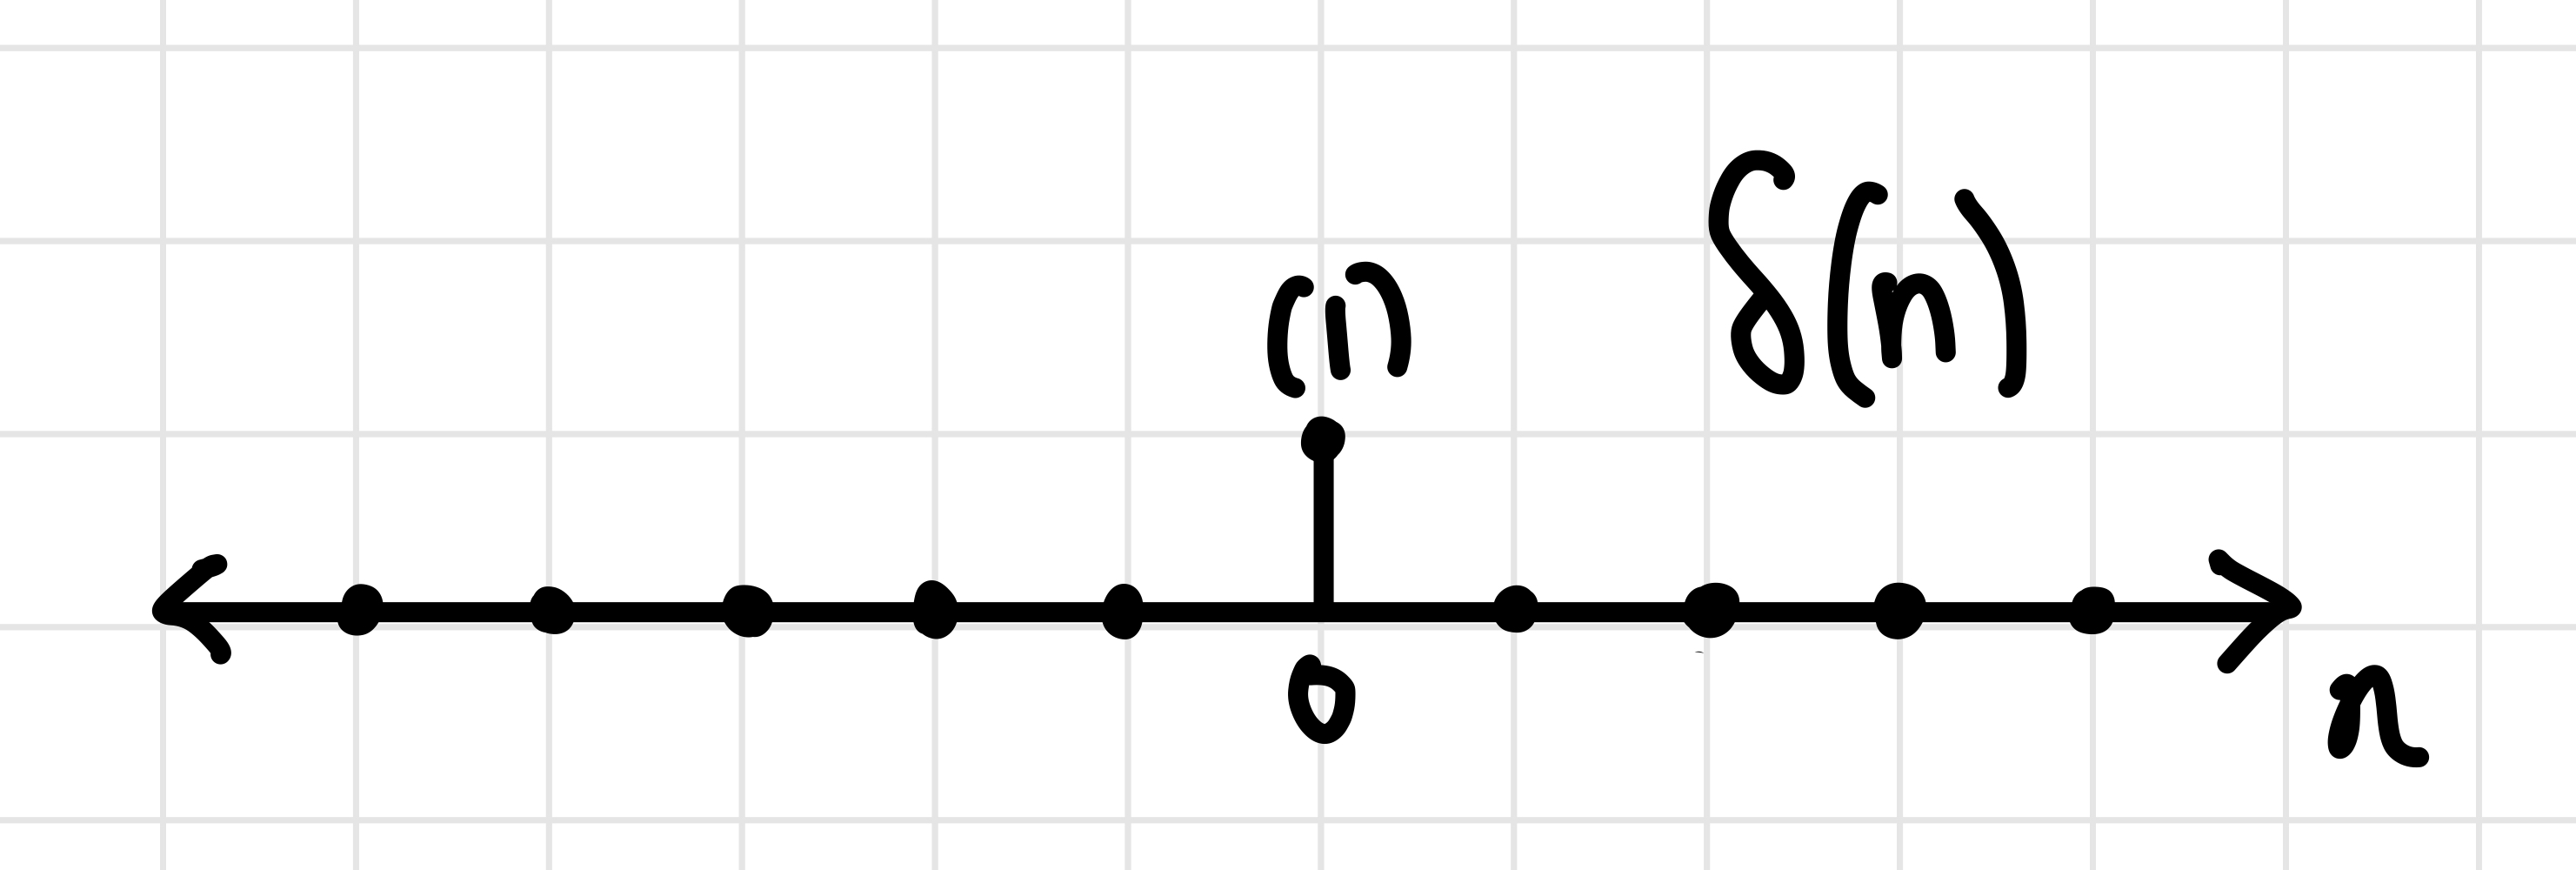
\includegraphics[ width=\textwidth/2]{lectures/img/Lec1_Delta.jpeg}
\end{center}
\[
    \delta(n) = \begin{cases}
                    1 &\text{if } n = 0\\
                    0 & \text{otherwise}
                \end{cases}
\]

Thus, we can express any DT signal in terms of a linear combination of shifted impulses.

\begin{center}
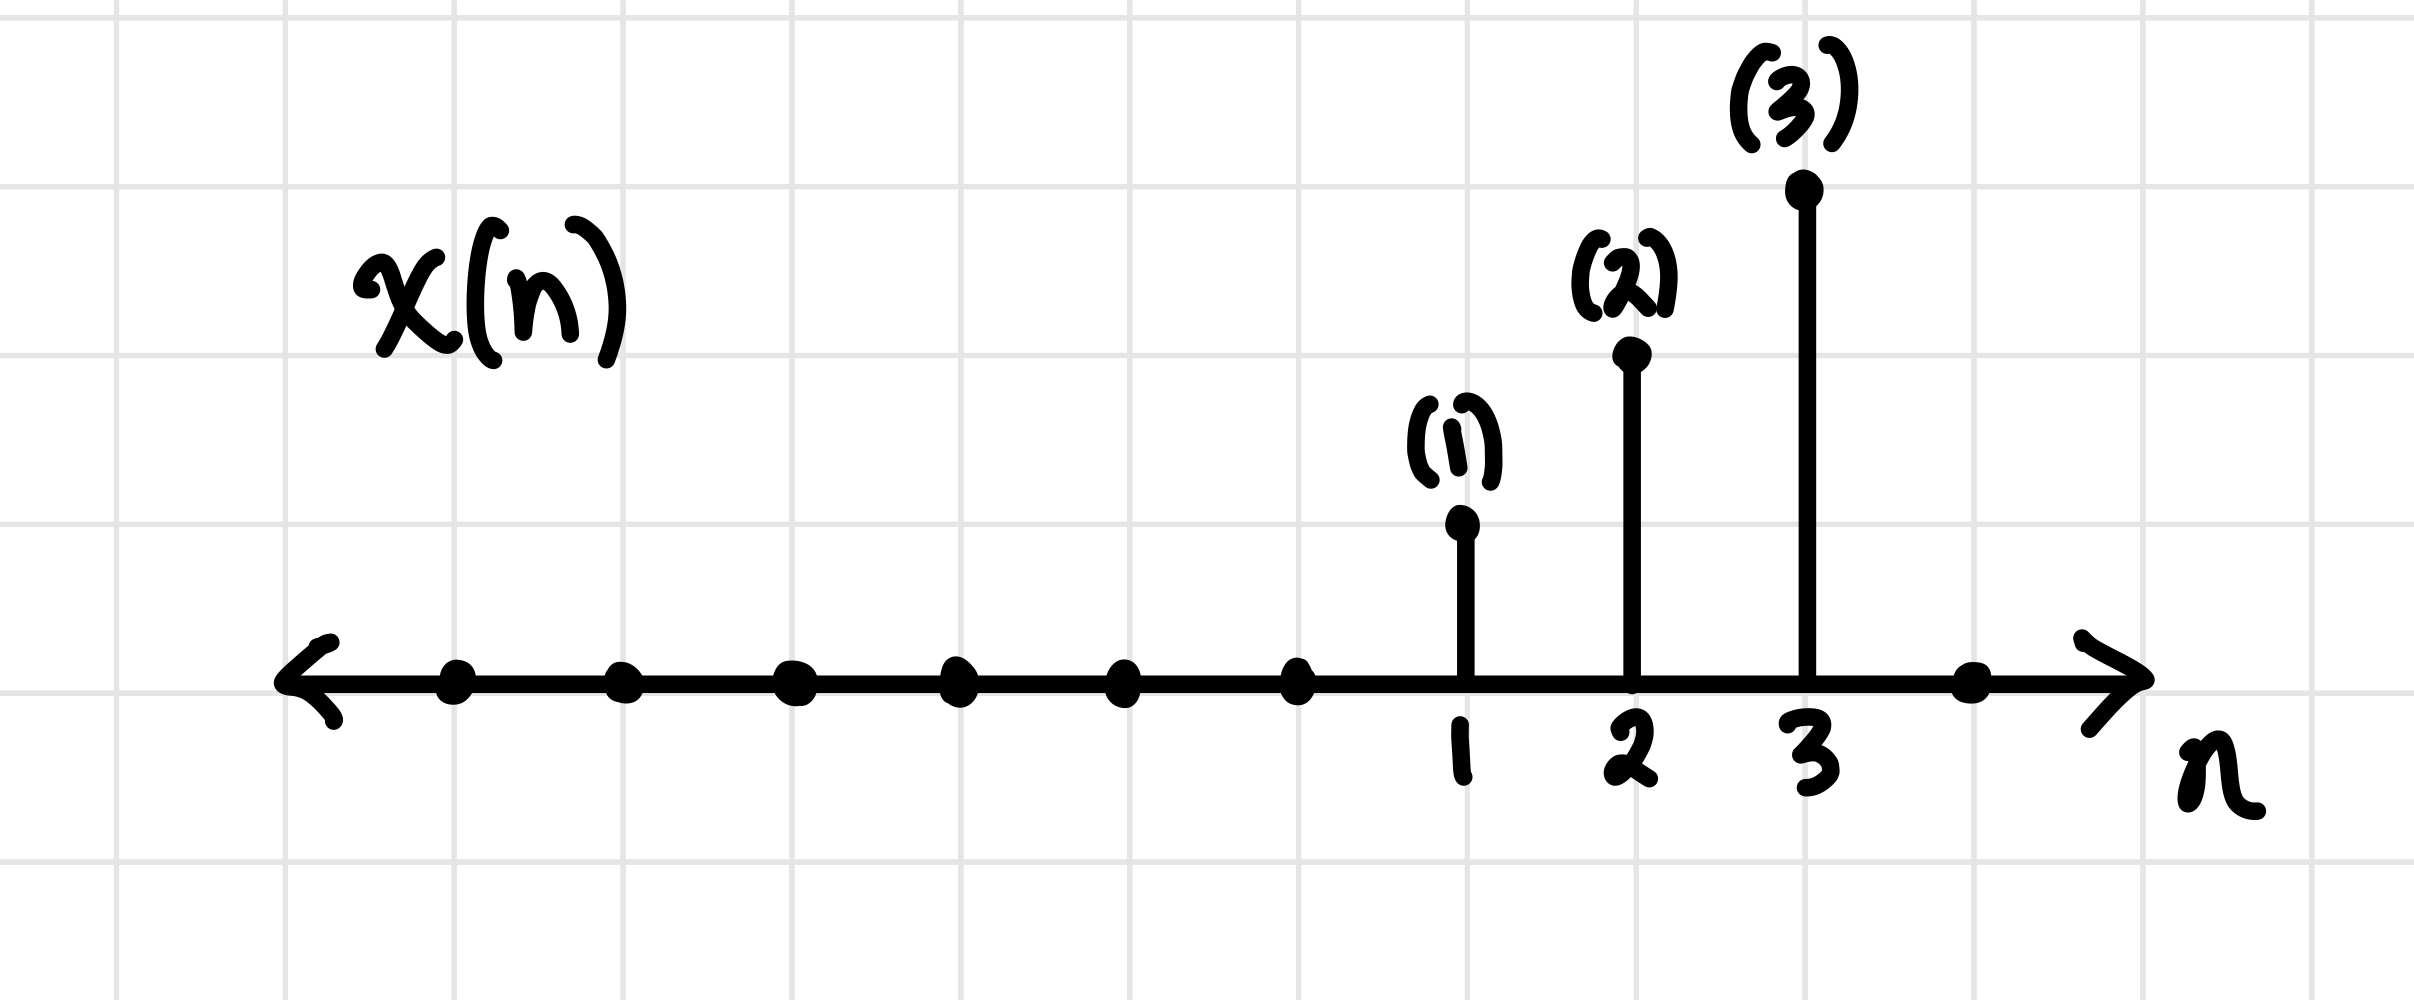
\includegraphics[ width=\textwidth/2]{lectures/img/Lec1_DeltaExample.jpeg}
\end{center}

\[x(n) = 1 \cdot \delta(n-1) + 2 \cdot \delta(n-2) + 3 \cdot \delta(n-3)\]

\subsubsection{DT Unit-Step Function}

\begin{center}
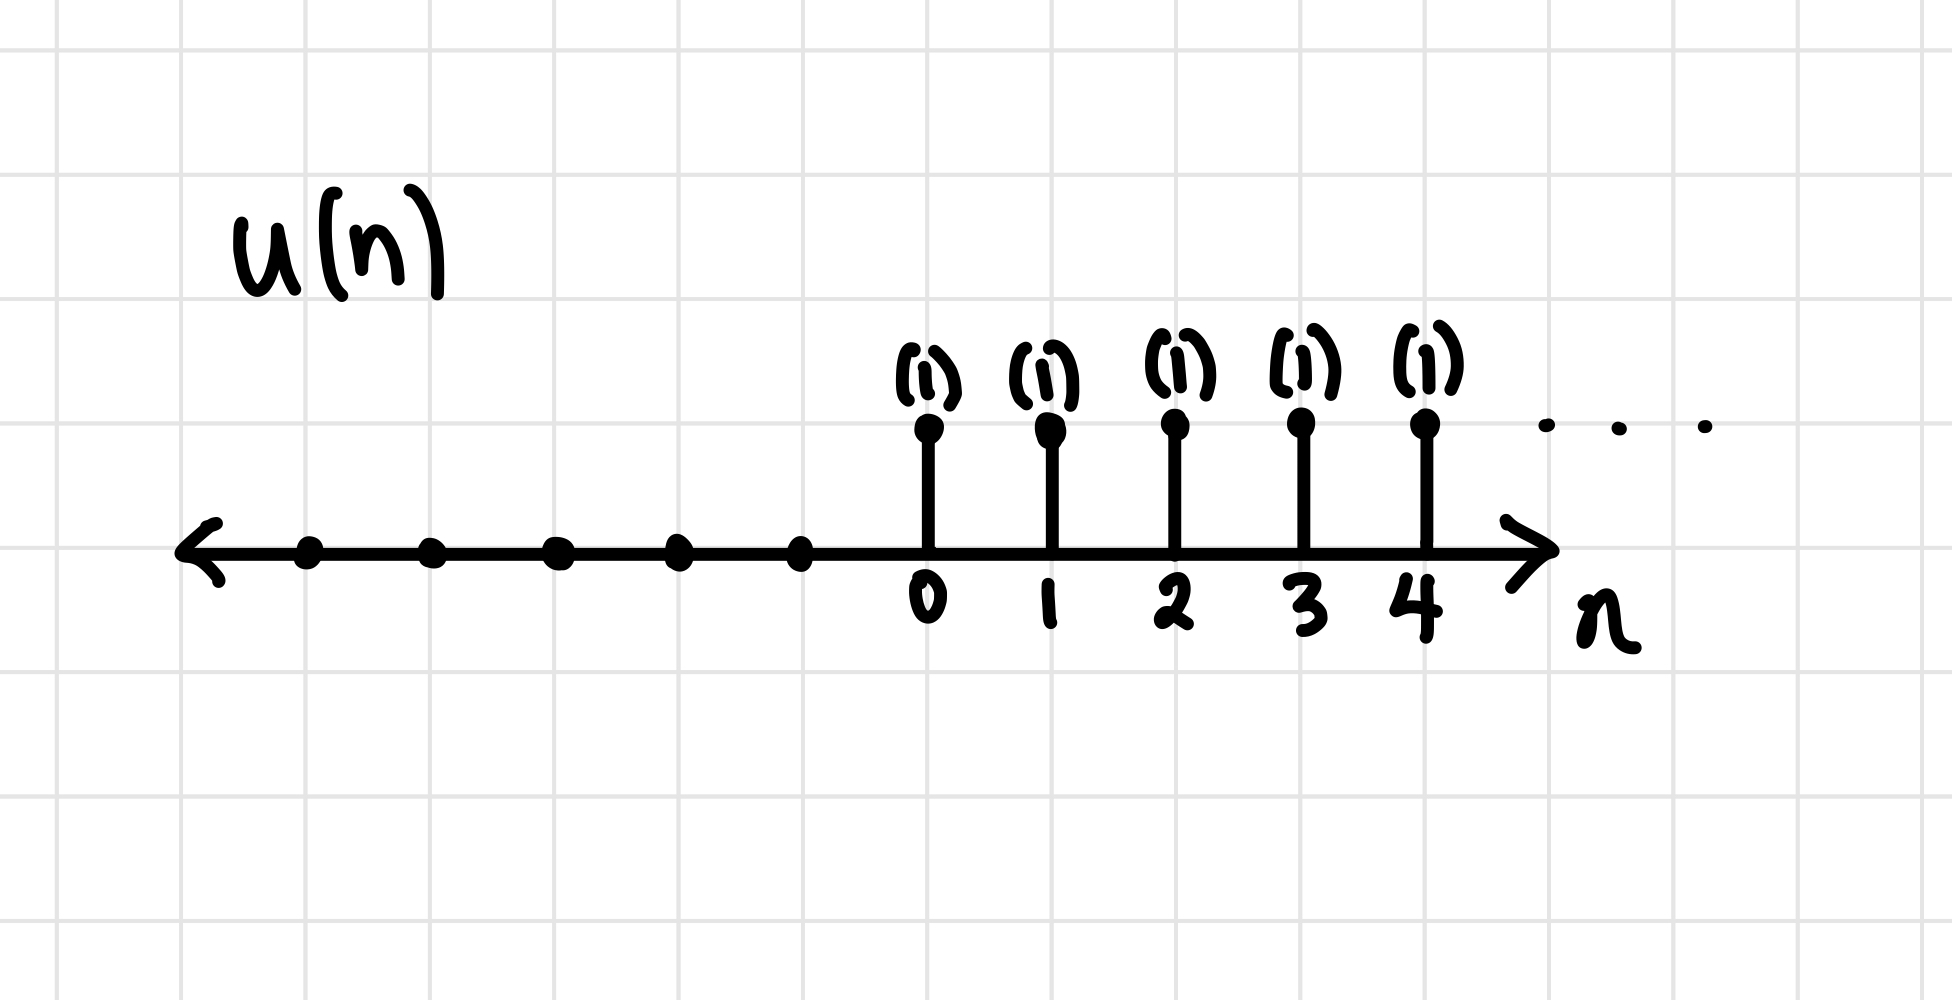
\includegraphics[ width=\textwidth/2]{lectures/img/Lec1_UnitStep.jpeg}
\end{center}

\[
    u(n)= \begin{cases}
    0 & \text{if } n < 0 \\
    1 & \text{if } n \geq 0
    \end{cases}
\]

We can actually express $u(n)$ in terms of shifted impulses ($\delta(n)$'s):
\begin{align*}
    u(n) &= \delta(n) + \delta(n-1) + \delta(n-2) + \cdots \\
    &= \sum_{k=0}^{\infty} \delta(n-k) \\
    &= \sum_{m = -\infty}^n \delta(m)
\end{align*}
Note that we do not use $i$ as an index variable since $i=\sqrt{-1}$.

Also, when we express $\delta(n)$ in terms of shifted $u(n)$, we get the following:
\[\delta(n)=u(n) - u(n-1)=\frac{u(n) - u(n-1)}{1}\]
This is a discrete-time derivative (slope).\textbf{ Impulse is the derivative of the unit step.} This will still hold in CT.

\subsection{Systems}

\textbf{Systems are also functions.
}

We can define system $F$ as a function/mapping between signal spaces $X$ and $Y$: \\
\[
\tikzmark{name}F: \tikzmark{a}X \to \tikzmark{b}Y
\] 
\begin{tikzpicture}[remember picture,overlay]
\draw[<-] 
  ([shift={(2pt,-2pt)}]pic cs:a) |- ([shift={(-10pt,-10pt)}]pic cs:a) 
  node[anchor=east] {Input Signal Space};
\draw[<-] 
  ([shift={(2pt,-2pt)}]pic cs:b) |- ([shift={(14pt,-10pt)}]pic cs:b) 
  node[anchor=west] {Output Signal Space};
\end{tikzpicture}

The systems we deal with in this class are \textbf{Single-Input, Single-Output (SISO)} systems.

Note that the inputs and outputs to $F$ are \textbf{signals}, i.e. functions. For example, $F$ may map $x_1(t) = \cos(t)$ to $y_1(t) = \sin(3t)$ where $x_1 \in X, y_1 \in Y$. Thus, we can think of the system $F$ as a mapping between sets of functions. Note that by definitions of functions, the entirety of the domain must be covered.

If $X = [\mathbb{R} \rightarrow \mathbb{R}]$ (i.e. space of real-valued CT signals) and $Y = [\mathbb{R} \rightarrow \mathbb{R}]$, then \textbf{$F$ is a Continuous-Time (CT) System}.

If $X = [\mathbb{Z} \rightarrow \mathbb{R}]$ (i.e. space of real-valued DT signals) and $Y = [\mathbb{Z} \rightarrow \mathbb{R}]$, then \textbf{$F$ is a Discrete-Time (DT) System}.

\subsubsection{Linearity}
Suppose we have a system $F: X \rightarrow Y$. We say that $F$ is linear if for all $x_1, x_2 \in X$, the following two properties hold:
\begin{align*}
    \text{Homogeneity/Scaling} & : F(\alpha x_1) = \alpha F(x_1) \\
    \text{Additivity} & : F(x_1 + x_2) = F(x_1) + F(x_2)
\end{align*}
This is also known in physics as superposition.

Next Time:
Time Invariance
